\documentclass[12pt,a4paper]{article}

%

\usepackage{amsmath}
\usepackage{amsfonts}
\usepackage{amssymb}
\usepackage[utf8]{inputenc}
\usepackage[T1]{fontenc}
\usepackage[brazilian]{babel}
\usepackage{mathpazo}
\usepackage[top=3cm,left=3cm,bottom=2cm,right=2cm]{geometry}
\usepackage{graphicx}
\usepackage{float}

%

\begin{document}
\thispagestyle{empty}
\begin{figure}\centering

\includegraphics[width=2.3cm,height=2.3cm]{if.jpg}
\end{figure}
\begin{center}\textbf{\large{INSTITUTO FEDERAL DE EDUCAÇÃO, CIÊNCIA E TECNOLOGIA DO MARANHÃO}}\end{center}
\vspace{3cm}

\begin{center}ENGENHARIA INDUSTRIAL ELÉTRICA\vspace{1.5cm}\\\textbf{DOUGLAS VIANA BERNARDINO} (EEI.180303)\end{center}
\vspace{3cm}

\begin{center}\textbf{CONCEPÇÃO DE CIRCUITOS DIGITAIS}\end{center}
\vspace{1.7cm}

Profº: José Iran Saraiva da Silva
\vfill \begin{center}\textbf{Imperatriz \\ 2018}\end{center}

\newpage %

\thispagestyle{empty}
\section*{Agradecimentos}
Meus sinceros agradecimentos:\\
\indent À  minha mãe, Maria do Rosário,  por ter ajudado no meu desenvolvimento pessoal e social durante minha adolescência.\\
\indent Ao meu pai, Gilson e sua esposa, Silbene,  por direcionarem minhas escolhas no que tange à educação.\\
\indent Ao meu professor, José Iran, por repassar seus conhecimentos de forma tão direta e concisa.

\newpage %

\section*{Resumo}

Os circuitos digitais são estão se tornando cada vez mais inerentes à tecnologia devido seus aspectos como praticidade e, principalmente, rapidez e portabilidade. Neste trabalho é apresentado um circuito digital desenvolvido em VhsicHDL, cujo o mesmo foi desenvolvido a partir de vários outros subcircuitos. De maneira pouco criteriosa, pode-se dizer que este circuito recebe um valor em binário de até 10 bits. Então este valor é decrementado consoante às ocorrências do fenômeno de bordas ascendentes do clock\footnote{Clock é o sinal de temporização usado em uma transmissão síncrona. Genericamente, ele é uma fonte de sinal de temporização para sequenciamento de eventos.}.

\newpage %

\section*{Abstract}
The digital circuits are are becoming increasingly inherent to the technology due to its aspects like practicality and mainly, speed and portability. This work presents a digital circuit developed in VhsicHDL, which has been developed from several other subcircuits. In a non-judgmental way, it can be said that this circuit receives a binary value of up to 10 bits. Then this value is decremented according to the occurrences of the rising edge phenomenon of the clock \footnote[1] {Clock is the timing signal used in a synchronous transmission. Generally, it is a timing signal source for event sequencing.}.

\newpage %

\section{Decrementador}
Para a construção do circuito principal, são necessários vários subcircuitos, e um deles é um circuito decrementador\footnote{Na Fig. 1, o mesmo pode ser identificado como sendo o bloco "Sub1\_structural".}. Abaixo pode-se observar uma visão geral do circuito principal.
\begin{figure}[h]\centering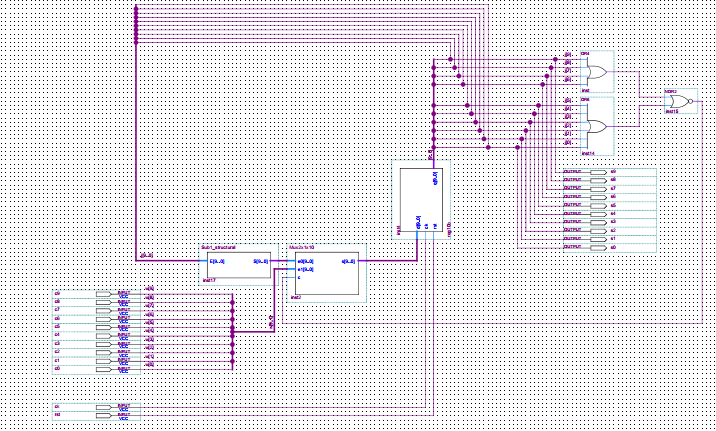
\includegraphics[scale=0.8]{circuit.png}\\ \caption{Circuito final completo.}\label{img:circuit}\end{figure}

\par Para fins de conclusão do exercício passado pelo professor, serão abordadas duas formas de construção do decrementador
\newpage
\subsection{Decrementador em nível estrutural}

É sabido que para ser feita a estrutura de um decrementador, é necessário usar uma propriedade similar à uma propriedade do conjunto natural $ x-y = x+(-y)$ \footnote{Os conjuntos numéricos possuem certas propriedades que são \emph{algébrica}, de \emph{ordem} e de \emph{completude}. Esta referência diz respeito à propriedade algébrica.}. Isto significa que devemos \emph{somar o número à ser decrementado com $-1$}. O único modo de fazer isso é escrevendo o $-1$ em forma de complemento de 2, e só então realizar a soma. O circuito que realiza esse comportamento é mostrado a seguir.
\begin{figure}[h]
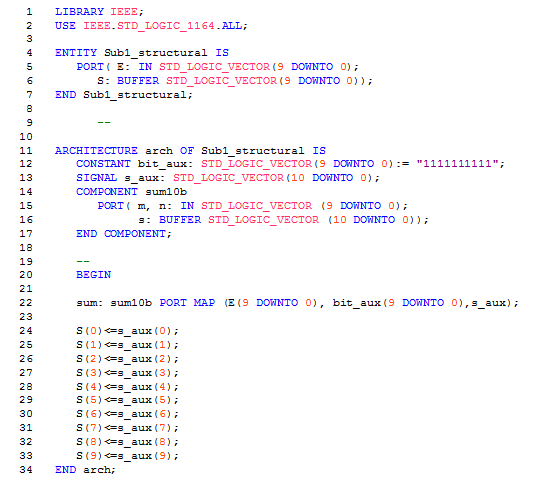
\includegraphics{fig2.png}
\caption{Decrementador em nível estrutural.}
\label{fg:decrementador_estrutural}
\end{figure}

Observe que para criar este circuito foi necessário um componente chamado "sum10b\footnote{Somador de dois conjuntos de 10 bits cada.}", cujo não será abordado pois isto faria com que fugíssemos do escopo deste trabalho.

\newpage
\subsection{Decrementador em nível comportamental}

Bem mais fácil de ser elaborado que o decrementador em nível estrutural é o de nível comportamental. A ideia principal consiste em subtrair '1' do vetor de entrada. Para ficar cláro, veja a descrição a seguir.\begin{figure}[h]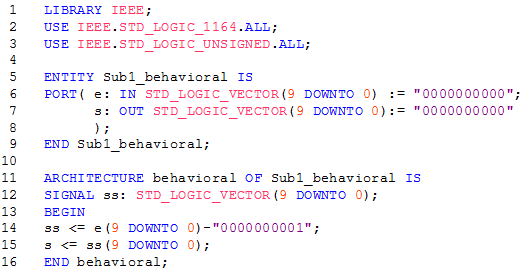
\includegraphics{fig3.png}\caption{Decrementador em nível comportamental.}\label{fg:decrementador_comportamental}\end{figure}


A figura a seguir ilustra a forma de onda dos dois tipos de decrementadores, ora pois, são circuitos equivalentes mesmo que tenham níveis diferentes de abstração.



\end{document}